\chapter{Evaluation}\label{chapter:Evaluation}
For the evaluation of the algorithms, some parameters need to be chosen in order to get reasonable results. Therefore, the edge-weight distribution is always set to be a uniform distribution on $[0.1, 1.1]$. As long as not mentioned differently, the number of graphs per algorithm is 3 and $n = 20, r = 3, d = 3, k = 2$. The choices of the parameters are justified in the respecting sections. In this chapter, especially in the plots, the term "approximation algorithm" refers to \cref{alg:ses}, whilst with "brute-force algorithm" usually \cref{alg:brute_force_size_just_one_side} is meant.



\section{Input graph sizes}
For evaluating the implementation of \cref{alg:ses} in comparison to the brute-force solution, the maximal size of graphs (in $n$) which can be brute-forced in a reasonable time is determined. The results for different number of vertices can be seen in \cref{fig:no_vertices_time}. In general, it is favourable to generate as large as possible graphs in order to see how the algorithm performs.
However, the as the brute-forcing time correlates with around $ \mathcal{O}(2^n)$, with the available resources, for $n=20$ brute-forcing already takes around $18$ s compared to $38$ s for computing a small expansion set with \cref{alg:ses}. As the brute-forcing time roughly doubles for each additional vertex, it is unfeasible to set $n$ much higher. Even though 21 vertices would be possible, due to \cref{eq:ndmr} an uneven number would unnecessarily limit the possible combinations of ranks and degree as evaluated in \cref{fig:rank_degree_times}, as for example, there would be no integer value for $m$ if $n = 21$, $d= 3$ and $r = 6$.

Aditionally, for analyzing the constant $C$ in \cref{fact:small_xi}, a plot of as many graps as possible seems to be ideal. So not only for brute-forcing but also for executing the estimation algorithm, the graph should not be too big. In conclusion, half a minute seems to be a reasonable time for one run of the algorithm. % as the time complexity of the small set expansion approcximation implementation shows to be at around ... $n...$
Therefore, $n$ is set to be 20 for further analysis.

\begin{figure}[htpb]
	\centering
	\includegraphics[scale=0.8]{figures/number_vertices_all_logs.pdf}
	\caption[Plot graph size against time]{Plot of the number of vertices $n$ in the graphs against the time for computing solutions. It can be seen that the brute-force algorithm takes a long time for larger graphs, while the approximation algorithm's time only increases slowly.\label{fig:no_vertices_time}}
\end{figure}


\section{Rank degree combinations}

As the graphs generated by the algorithms have uniform ranks and  regular degrees (except those generated by \cref{alg:GenerateRandomGraphWithResampling}), it needs to be determined which combination of $r$ and $d$ should be chosen. As already mentioned, because of \cref{eq:ndmr} they can not be chosen freely, since not for all combinations $r$-uniform $d$-regular graphs exist on $n$ vertices, as $m$ might not be integer. 
As all of the variables need to be non-negative integers, one can ensure to never violate that constraint for any $n$ by setting $d=r$. An evaluation of the time constraints can be seen in \cref{fig:rank_degree_times}. Interestingly, for equal $r$ and $d$, the brute-force algorithm's time did almost not increase when $(d,r)$ was increased from $(2,2)$ to $(8,8)$. The small set approximation algorithm's times however, seem to increase linearly with $r$ and $d$. For other combinations, interestingly the brute-force algorithm needed more time for comparatively high $\frac{d	}{r}$ ratios.

For easier evaluation of the other properties, the rank and degree were chosen to be $r=3$ and $d=3$, as with a rank of $3$ it is explicitly demonstrated that the algorithms work on hypergraphs.
\begin{figure}
	\centering
	\includegraphics[scale=0.8]{figures/rank_degree_combinations_all_logs.pdf}
	\caption[Plot times rank degree combinations]{Plot of times for rank degree combinations.\label{fig:rank_degree_times}}
\end{figure}


\section{Evaluation of k}

The value of $k$ plays an important role in the properties of the graph as well as the runtime. As described in \cref{alg:procedural_minimizer}, $k$ vectors are constructed.
As for $k = 1$, no SDP must be solved, the algorithm terminates quickly. However, this does not make sense anyways, as the spectral properties of the graph would not be taken advantage of, as in \cref{alg:procedural_minimizer}, for $k=1$, only the unit vector would be returned.
As seen in \cref{fig:k_time}, for higher $k$, the time for each small expansion set approximation increases. Profiling the algorithm also showed that most of the time was spent on solving the SDP. Unfortunately for higher $k$s, sometimes the optimization takes unreasonably long, presumably due to numerical instabilities.

\begin{figure}
	\centering
	\includegraphics[scale=0.8]{figures/k_all_logs.pdf}
	\caption[Plot k time ]{Plot of $k$ against time for the approximation algorithm.\label{fig:k_time}}
\end{figure}

\section{Small expansion sizes}

As seen in \cref{fig:sizes_small_expansions}, most of the sampled small expansion sets have a small number of vertices. TODO: verify: As k increases, this trend continues, going along the trend of getting smaller sets for larger k as indicated in \cref{fact:small_xi}.


Since higher values of $k$ were not feasible in \cref{eq:small_expansion} due to numerical issues of the implementation as well as time constraints, the upper limit of the expansion size $|S|<\frac{24|V|}{k}$ in \cref{fact:small_xi} can not be verified as $k<5$ here.

One aspect which might be noted is that most of the expansions have size $1$, which does not prove any insight, as the expansion of every subset $S$ with just one vertex $v\in S$ takes value $1$, as $\delta S = w_v = w(S)$ (if every edge contains at least two vertices). In a real-world application of this algorithm, these sets might be discarded.


TODO plot of k=2, k=3

\begin{figure}
	\centering
	\includegraphics[scale=1]{figures/quality_evaluation_log_small_expansion_sizes.pdf}
	\caption[Plot sizes small expansions]{Plot of sizes of small expansions.\label{fig:sizes_small_expansions}}
\end{figure}


\section{Random graphs comparison}
As the expansion for non-connected graphs is always $0$, which is not interesting, only algorithms which guarantee to return connected graphs are considered, namely \ref{alg:GenerateRandomGraphWithResampling}, \ref{alg:swap_edges} and \ref{alg:spanning_tree}.

The expansion of the graphs is evaluated against each other via brute-force. The results can be seen in \cref{fig:plot_lowest_expansion_each_size}. Interestingly, no big differences in the expansion values can be determined. The average expansion value of \ref{alg:GenerateRandomGraphWithResampling} was slightly higher than the value of \ref{alg:swap_edges} and \ref{alg:spanning_tree}, which might be the case because \ref{alg:GenerateRandomGraphWithResampling} did return non-regular graphs.

\begin{figure}
	\centering
	\includegraphics[scale=1]{figures/creation_algorithm_log_lowest_expansion.pdf}
	\caption[Plot lowest expansion for different algorithms]{Plot of the lowest expansion values of graphs created by different algorithms for each size of the expansion set. For the calculaion \cref{alg:brute_force_size} was utilized.\label{fig:plot_lowest_expansion_each_size}}
\end{figure}

\section{Estimation of C}
As according to \cref{fact:small_xi} a small value of C would be favourable to ensure that the expansion sets generated by \cref{alg:ses} have small expansions values. 
For estimating $C$, the inequality of \cref{fact:small_xi} can be changed to:
\begin{equation} \label{eq:c_estimate}
C\ge \frac {\phi(S)}{ \min\{\sqrt{r \log k}, k \log k  \log \log k \sqrt{\log r} \} \cdot \sqrt{\xi}}
\end{equation} Here, $\log$ refers to the natural logarithm, requiring a value of $k\ge3$. As for higher values of $k$ the at times the calculation takes very long, it is set to $k=3$ here.


However, the plot in \cref{fig:c_estimates} does not show a clear picture, as the calculated values for $ C$ of each run of \cref{alg:ses} lie between $0.38$ and $2.71$. However, one could hypothise that the value of $C$ indeed is not much bigger than $2.71$, since no bigger estimates appeared and most of the values were close to it. It might be a coincidence, but the value is similar to Euler's number $e$, which might give some inspiration for further proofs on upper bounds of $C$. 
However, for higher confidence, this should be tested on a large scale, especially with higher $k$ and other combinations of the other parameters and graph construction algorithms.


\begin{figure}
	\centering
	\includegraphics[scale=1]{figures/quality_evaluation_log_C_estimates.pdf}
	\caption[Plot C estimates]{Plot of estimates for the constant C in \cref{fact:small_xi}.\label{fig:c_estimates}}
\end{figure}





\section{Comparison of expansion values}




Finally, the quality of the expansion values is analyzed. Here it seems reasonable to compare only expansion sets of the same size with another. As seen in \cref{fig:expansion_approx_vs_brute}, the lowest expansion value found by the brute force algorithm is, as expected, always at least as low as the value achieved by the small expansion set found by the approximation algorithm. However, when comparing the best expansion values, found in $100$ repetitions of the steps after solving the SDP in \cref{alg:lg:ses}, against the best one-percentile of values as found by the brute-force algorithm, the approximation algorithm performs better in around 21\% of times, even though that is not the aim of the approximation algorithm. Compared to the average brute-foce value, which is the average expansion over all sets, it can be seen that the approximation algorithm performs significantly better than random guessing, as most of the entries lie above the line. The same can be seen when the median expansion value is considered, which is a positive result. 

As the performance of the algorithm is now evaluated, possible applications can be discussed in the next chapter.


\begin{figure}
	\centering
	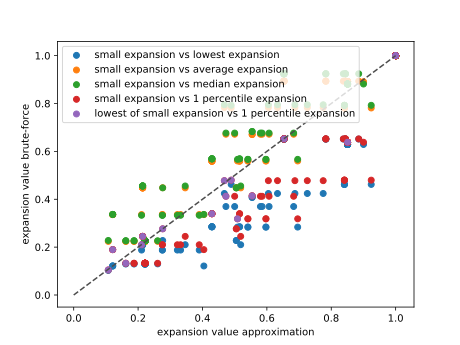
\includegraphics[scale=1]{figures/quality_evaluation_log_expansion_values_for_same_number_verticies.pdf}
	\caption[Plot expansions approximation vs brute force]{Plot of the expansion values achieved by the small expansion set approximation algorithm against the expansion set of the same size with the lowest expansion (as generated through the brute-force approach).  Entries below the line signal that the expansion found by the approximation algorithm was worse than the set found by the brute force algorithm. \label{fig:expansion_approx_vs_brute}}
\end{figure}




